\documentclass{mc2015}
%%%%%%%%%%%%%%%%%%%%%%%%%%%%%%%%%%%%%%%%%%%%%%%%%%%%%%%%%%%%%%%%%%%%%
\usepackage[T1]{fontenc}         % Use T1 encoding instead of OT1
\usepackage[utf8]{inputenc}      % Use UTF8 input encoding
\usepackage{microtype}           % Improve typography
\usepackage{booktabs}            % Publication quality tables
\usepackage{amsmath}
\usepackage{graphicx}
\usepackage{float}
\usepackage[exponent-product=\cdot]{siunitx}
\usepackage[colorlinks,breaklinks]{hyperref}
\hypersetup{linkcolor=black, citecolor=black, urlcolor=black}
%%%%%%%%%%%%%%%%%%%%%%%%%%%%%%%%%%%%%%%%%%%%%%%%%%%%%%%%%%%%%%%%%%%%%

\usepackage{lipsum}
\usepackage{amsmath}
\usepackage{array}
\usepackage{color}
%\usepackage{graphicx}
%\usepackage{float} % utiliser H pour forcer a mettre l'image ou on veut
\usepackage{lscape} % utilisation du mode paysage
\usepackage{mathbbol} % permet d'avoir le vrai symbol pour les reels grace a mathbb
\usepackage{enumerate} % permet d'utiliser enumerate
\usepackage{moreverb} % permet d'utiliser verbatimtab : conservation la tabulation
\usepackage{stmaryrd} % permet d'utiliser \llbrackedt et \rrbracket : double crochet
\usepackage[noabbrev]{cleveref} % permet d'utiliser Cref and Cref
\usepackage{caption} % permet d'utiliser subcaption
\usepackage{subcaption} % permet d'utiliser subfigure, subtable, etc
%\usepackage[margin=1.in]{geometry} % controle les marges du document
\usepackage{algorithm}
\usepackage{url}


\newcommand\bn{\boldsymbol{\nabla}}
\newcommand\bo{\boldsymbol{\Omega}}
\newcommand\br{\mathbf{r}}
\newcommand\la{\left\langle}
\newcommand\ra{\right\rangle}
\newcommand\bs{\boldsymbol}
\newcommand\red{\textcolor{red}}
\newcommand\ldb{\{\!\!\{}
\newcommand\rdb{\}\!\!\}}
\newcommand\llb{\llbracket}
\newcommand\rrb{\rrbracket}

\renewcommand{\(}{\left(}
\renewcommand{\)}{\right)}
\renewcommand{\[}{\left[}
\renewcommand{\]}{\right]}

%%%%%%%%%%%%%%%%%%%%%%%%%%%%%%%%%%%%%%%%%%%%%%%%%%%%%%%%%%%%%%%%%%%%%
% Insert authors' names and short version of title in lines below

\authorHead{Bruno Turcksin}
\shortTitle{Parallel $S_n$ Sweeps on Adapted Mesh}

%%%%%%%%%%%%%%%%%%%%%%%%%%%%%%%%%%%%%%%%%%%%%%%%%%%%%%%%%%%%%%%%%%%%%

\begin{document}
\title{Parallel $S_n$ Sweeps on Adapted Mesh}
\author{Bruno Turcksin} 
\affil{Department of Mathematics \\
  Texas A\&M University \\
  3133 TAMU, College Station, TX 77843-3133 \\
  turcksin@math.tamu.edu
}

\maketitle

\begin{abstract}
  We study parallel sweeps on adaptively refined meshes. Unlike on regular
  grids, there is no known optimal parallel sweeps on unstructured mesh and
  thus, multiple heuristics have been proposed over the years. In this paper, we
  study the CAP-PFB (Cut Arc Preference - Parallel Forward Backward) algorithm
  on regular grids and adaptively refined meshes. We begin by recalling the
  CAP-PFB heuristic, then we explain how it can be applied on adapted meshes.
  After that, we compare the sweeps produced by different initial sweeps on
  regular and adapted meshes. We show that on regular grids, CAP-PFB finds an
  optimal sweep independently of the initial sweep used. On adapted meshes, the
  best results are obtained when using a serial initial sweep for CAP-PFB. This
  is somewhat unexpected that the ``worst'' initial sweep lead to the best
  result. We conclude that a good initial sweep for CAP-PFB should take into
  account the interaction of sweeps along different directions before trying to
  minimize the number of stages.

  \emph{Key Words}: transport sweeps, parallel transport, AMR
\end{abstract}

% In the paper, they gave a weight of 1/3 instead of zero to the arcs between
% two different processors.
\section{Introduction}

When discretizing the angular variable of the transport equation with the
discrete ordinates method, it is usually necessary to perform multiple transport
sweeps through the mesh. A transport sweep (or simply a sweep for short)
directly inverts the steaming-plus-collision operator of the transport equation,
i.e., it solves for every angle:
\begin{equation}
  \bo_m\cdot\bn\Psi_{m,g}^{(k+1)}+\sigma_{t,g}\Psi_{m,g}^{(k+1)} =
  q_{m,g}^{(k)}
  \label{task}
\end{equation}
where $\Psi_{m,g}^{(k+1)}$ is the angular flux, $q_{m,g}^{(k)}$
is the sum of the volumetric source with the scattering source computed using
the angular fluxes from the
previous iteration (denoted by the superscript $k$), $m$ is the index associated
with the angle $\bo_m$, and $g$ is the index of the energy group. If the
incident angular flux is known on the boundary of the domain and there are no
reflecting or periodic boundaries, the dependency graph associated with the
sweep through a mesh along a direction is a directed and acyclic graph (DAG),
see \Cref{tasks}.
\begin{figure}[H]
  \begin{subfigure}[c]{.5\textwidth}
    \centering
    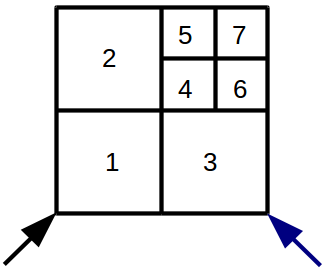
\includegraphics[width=5cm]{task_1}
  \end{subfigure}
  \begin{subfigure}[c]{.5\textwidth}
    \centering
    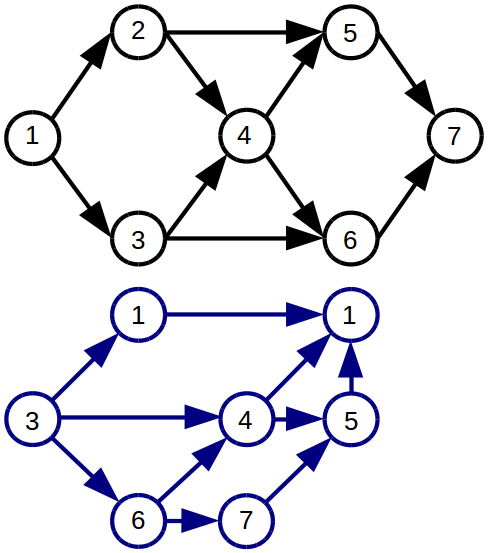
\includegraphics[width=5cm]{task_2}
  \end{subfigure}
  \caption{Mesh and DAG associated to the sweep along two different directions.}
  \label{tasks}
\end{figure}

Sweeping through a mesh in parallel can be viewed as a resource-constrained
project scheduling problem (RCPSP) \cite{Brucker1999,Kolisch2006} where the
constraints are given by multiple DAG (one for each direction) and by the fact
that a processor cannot execute two tasks (vertices of the DAG) at the same
time. The goal of RCPSP is to schedule the tasks such that all the constraints are
satisfied and that the time required to execute all the tasks is minimal. 
RCPSP has been extensively studied for more than four decades
\cite{Pritsker1969} but most sweeping algorithms have been developed
independently of these researches. In this paper, a task consists of solving
\cref{task} for a given direction and a given energy group on a cell or a group
of cells.

When studying sweeping algorithms, it is also necessary to study the
partitioning of the mesh. Two identical meshes partitioned differently will lead
to different optimal scheduling. Therefore, to obtain the best speed up, given a
mesh and a number of processors, the sweeping algorithm and the partitioning
should be studied together. However, here we will assume that the
partitioning is given. This is representative of the case where the partitioning
is done by a third-party library or when the partitioning cannot be tailored for
the transport equation because other physics must be accounted for. In
\cite{Adams2013}, a family of optimal sweeping algorithms is described for
regular grids. For unstructured grids, several heuristics have been proposed
over the years
\cite{Pautz2002,Plimpton2005,Yan2013,Colomer2013,Kumar2005,Mo2014}. In this
paper, we study the CAP-PFB algorithm introduced in \cite{Mo2014} which is based
on a widely used method in RCPSP \cite{Li1992}. In particular, we will study how
the algorithm behaves on regular grids and on meshes constructed using adaptive
mesh refinement (AMR)
\cite{Arnold2000,Baker2002,Bangerth2007,Jessee1998,Wang2010a}. This work will
show some preliminary results on the performance of the sweeping algorithm on 
meshes similar to
the ones produced by deal.II \cite{Bangerth2007,Bangerth2013} and p4est
\cite{Burstedde2011}. Deal.II is an open source finite element library which
uses the p4est library for the partitioning. The rest of this paper is organized
as follows: in \Cref{parallel_sweeps}, we explain the CAP-PFB algorithm
introduced in \cite{Mo2014} and we show how to apply it to adapted meshes. In
\Cref{results}, we compare the results obtained with CAP-PFB using different
initial sweeps, on uniform meshes where the optimal solution is known
\cite{Adams2013} and on meshes more typical of what is obtained using AMR.
We end with our conclusions in \Cref{conclusions}.


\section{Parallel sweeps on AMR mesh} \label{parallel_sweeps}

\subsection{CAP-PFB algorithm}

In this Section, we explain the CAP-PFB (Cut Arc Preference - Parallel Forward
Backward) algorithm introduced in \cite{Mo2014}. We will start with the general
Forward-Backward (FB) algorithm \cite{Li1992}. This algorithm has been developed
to schedule a set of tasks given dependencies between the tasks and constraints
on the resources. It is based on the observation that when we try to execute the
tasks as soon as possible, a lot of work is done at the beginning of the
schedule but it quickly decreases to only few tasks later
on. The opposite is true when we try to execute the tasks as late as possible;
few tasks are performed at the beginning but a lot are done at the end
of the schedule. The idea beyond the FB algorithm is to alternate a phase where the
tasks are scheduled as late as possible (backward iteration) with a phase where the
tasks are scheduled as early as possible (forward iteration)\footnote{The
original algorithm applied the forward iteration first.}. The hope is
that we will get a more constant distribution of the work and therefore,
decrease the time needed to execute all the tasks. The algorithm works as
follow:
\begin{algorithm}[H]
  \caption{FB algorithm}
  \begin{itemize}
    \item Start with an initial scheduling.
    \item Iterate until convergence or maximum number of steps:
      \begin{enumerate}
        \item Backward iteration:
          \begin{enumerate}
            \item Compute the ranks of the tasks based on the current scheduling.
            \item Sort the tasks in descending order of the ranks to create a
              new scheduling.
          \end{enumerate}
        \item Forward iteration:
          \begin{enumerate}
            \item Compute the ranks of the tasks based on the current
              scheduling, i.e. the scheduling produced by the backward
              iteration.
            \item Sort the tasks in ascending order of the ranks to create a new
              scheduling.
          \end{enumerate}
      \end{enumerate}
  \end{itemize}
  \label{fb}
\end{algorithm}
Different FB algorithms will differ by the method used to compute the ranks of the tasks. The
Cut Arc Preference (CAP) method uses DAG to represent the dependency of the
tasks and computes the ranks of the tasks using the cut arcs of the graph. Cut
arcs are arcs between tasks owned by different processors. The ranks are
computed as follows:
\begin{description}
  \item[Backward iteration:] the rank of a task is the earliest start time of all its downstream tasks
    owned by a different processor. Tied are broken using the task own start time.
    %$\min_{(v_k,v_j)\in S_i}\left\{s_j-w_{k,j}\right\} \cup \left\{+\infty\right\}$
  \item[Forward iteration:] the rank of a task is the latest end time of all its upstream tasks owned
    by a different processor. Tied are broken using the task own end time.
    %$\max_{(v_j,v_k)\in B_i} \left\{f_j+w_{j,k}\right\} \cup \left\{-\infty\right\}$
\end{description}
PFB works exactly like FB but it assumes that the tasks are distributed among processors.

\subsection{CAP-PFB on adapted mesh}

In \Cref{subdomain_id}, we show a mesh and its partitioning generated by deal.II and p4est 
on 16 processors. This is a typical mesh produced by these libraries and it is
representative of the case that we want to tackle (the problem solved here is a
simple Laplace equation but the mesh and the partition are rather typical). 

\begin{figure}[H]
  \begin{subfigure}[b]{.5\textwidth}
    \centering
    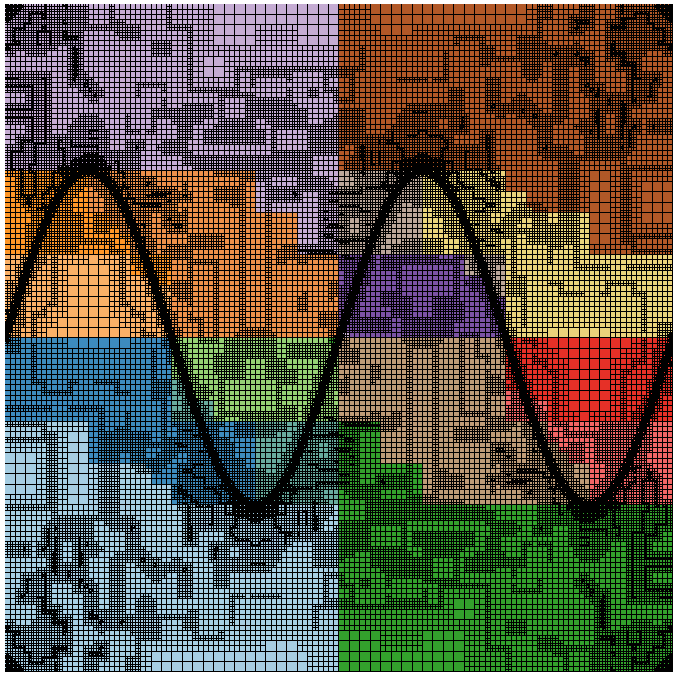
\includegraphics[width=5cm]{subdomain_id_0}
    \caption{Partitioning and mesh.}
  \end{subfigure}
  \begin{subfigure}[b]{.5\textwidth}
    \centering
    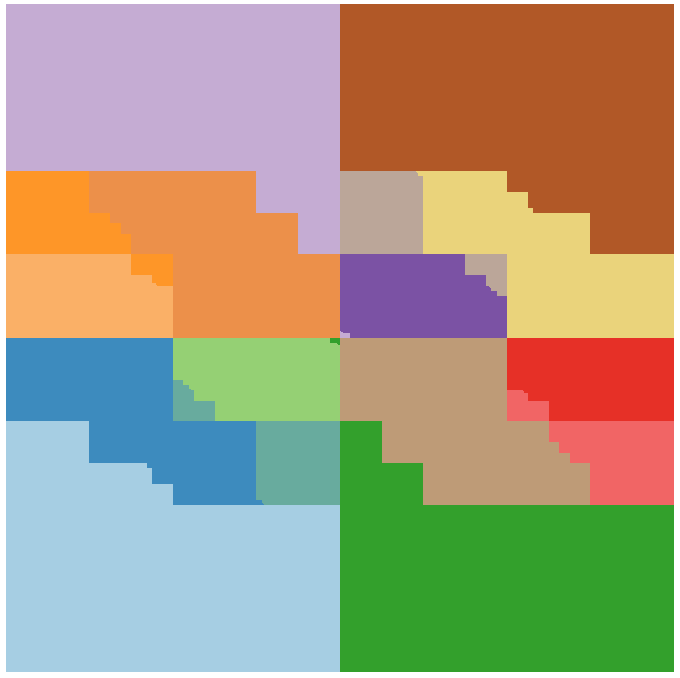
\includegraphics[width=5cm]{subdomain_id_1}
    \caption{Partitioning.}
  \end{subfigure}
  \caption{Partitioning and mesh using 16 processors (Step-40 of deal.II).}
  \label{subdomain_id}
\end{figure}

We can see in \Cref{subdomain_id} that the domain owned by each processor is not
convex and that some
processors own disjoint domains. In \cite{Mo2014}, the authors studied CAP-PFB
when all the tasks have the same amount of work to execute. In this case,
CAP-PFB is guarantee to converge to a scheduling which may or may not be
optimal. For the partition shown in \Cref{subdomain_id}, guaranteed convergence can be achieved by using
tasks that are associated to only one cell. However, this will create an
excessive amount of communication between processors which will negatively impact the performance
\cite{Pautz2002}. Therefore, it is necessary to have tasks that own more than
one cell. On a totally unstructured mesh, gathering cells to form convex zones
can be a difficult problem. However, this can be easily done on an AMR mesh since the
children of a coarse cell can be gather to form a convex zone, i.e. the parent
cell. It is of course necessary that all the children are owned by the same
processor. Otherwise, a task would span over multiple processors and
it would be impossible to compute its ranks. The coarsening step 
can be extended to grand-parent, great-grand-parent, etc. This process will create
tasks that have very different number of cells associated to them either
because some cells have less ancestors or because some cells that have a common
ancestor are owned by different processors. Having tasks containing different
numbers of cells can be taken into account in CAP-PFB but the resulting
algorithm loses its convergence property. We will show in \Cref{results} that
the number of stages, i.e. the number of steps needed to sweep through the mesh,
of successive scheduling oscillates.

\subsection{Initial sweeps}

In the next Section, we will compare the results of CAP-PFB using different initial sweeps:
\begin{description}
  \item[serial:] this sweep is the same as a serial sweep. We sweep through the
    mesh one
    direction at the time and at any given time only one task is executed. We
    will refer to it as \emph{serial}.
  \item[randoms:] two initial sweeps are generated randomly. We will refer to
    them as \emph{random1} and \emph{random2}
  \item[interleaved DFDS:] this sweep is defined in \cite{Pautz2002}. We will
    refer to it as \emph{iDFDS}. This heuristic prioritizes tasks that have
    downstream tasks on other processors. It is important to note that this algorithm was
    developed to deal with number of tasks much larger than what the tests in
    the next Section use.
\end{description}

\section{Results} \label{results}

In this Section, we examine the number of stages produced by the CAP-PFB
heuristic. In the first test, we compare the sweeps produced by CAP-PFB
with the optimal solution on a uniform mesh. In the second and third tests, we
look at the scheduling on AMR meshes. In all the tests, the domain is square and
we use a $S_8$ quadrature, i.e. 40 directions. 20 CAP-PFB iterations will be
performed for each initial sweep.

\subsection{Uniform mesh}

In this test, we compare the number of stages on a uniform two-dimensional mesh 
where each processors owns 40 tasks (one task for each direction). In this
setup, the optimal number of stages is given by \cite{Adams2013}:
\begin{equation}
  \mu = P_x + P_y - 4 + N_{\textrm{tasks}},
\end{equation}
\noindent with $P_x \times P_y$ the process grid and $N_{\textrm{tasks}}$ the number of
tasks that each processors has to execute. In \Cref{uniform}, we compare the number of
stages obtained using CAP-PFB to the optimal solution for different number of
processors.

% Order of results: no seed, seed = 0, seed = 1.
\begin{table}[H]
  \begin{center}
    \caption{Number of stages required to sweep through an uniform mesh.
      \emph{N. procs} is the number of processors ($P_x \times P_y$), \emph{Init. sweep} is the
      method used to produce the initial sweep, \emph{Init. n. stages} is the
      number of stages of the initial sweep, \emph{Best n. stages} is the
      number of stages of the best sweep computed, \emph{Optimal n. stages} is the
      number of stages of the optimal sweep, and \emph{Iter.} is the number
    of CAP-FBS iterations performed to reach \emph{Best n. stages}.}
    \begin{tabular}{|c|c|c|c|c|c|}
      \hline
      N. procs & Init. sweep & Init. n. stages & Best n. stages & Optimal n. stages & Iter. \\
      \hline
      $10\times 10$ & \emph{serial}  &   4000 &  56 &  56 & 1 \\
      $10\times 10$ & \emph{random1} &    155 &  56 &  56 & 2 \\
      $10\times 10$ & \emph{random2} &    153 &  56 &  56 & 1 \\
      $10\times 10$ & \emph{iDFDS}   &     56 &  56 &  56 & 0 \\
      $30\times 30$ & \emph{serial}  &  36000 &  96 &  96 & 1 \\
      $30\times 30$ & \emph{random1} &    392 &  96 &  96 & 2 \\
      $30\times 30$ & \emph{random2} &    376 &  96 &  96 & 2 \\
      $30\times 30$ & \emph{iDFDS}   &     96 &  96 &  96 & 0 \\
      $50\times 50$ & \emph{serial}  & 100000 & 136 & 136 & 1 \\
      $50\times 50$ & \emph{random1} &    570 & 136 & 136 & 2 \\ 
      $50\times 50$ & \emph{random2} &    573 & 136 & 136 & 2 \\
      $50\times 50$ & \emph{iDFDS}   &    136 & 136 & 136 & 0 \\
      \hline
    \end{tabular}
    \label{uniform}
  \end{center}
\end{table}

We can see that the heuristic converges to the optimal solution in only one or
two iterations for every initial sweep except for \emph{iDFDS}. \emph{iDFDS} 
finds the optimal scheduling without CAP-PFB. Even though the number of stages is
identical, the sweeps obtained using different initial sweeps are
different.

\subsection{First AMR test}

In this test, the cells in the middle of the domain are refined (\Cref{mesh_1}).
The red squares represent processors and the black squares represent cells
or sets of cells. 40 tasks, each one requiring one unit of work, are
associated with each black square.

\begin{figure}[H]
  \centering
  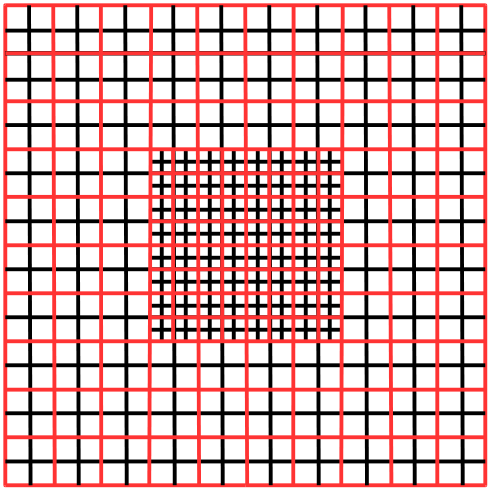
\includegraphics[width=5cm]{mesh}
  \caption{Mesh refined in the middle of the domain.}
  \label{mesh_1}
\end{figure}

First, we test the case where each processors owns 160 tasks (\Cref{amr_1}). For
this mesh the optimal number of stages is not know but we can obtained an
estimate of
the minimal number stages by counting the minimum number of stages before the
central processors can start working ($N_{fill}$) and the number of tasks own by
each of the central processors. In this case, we get: the minimal numbers of stages
(\emph{Minimal n. stages}) equals $2\times N_{fill}+N_{tasks}$ \cite{Adams2013}.

% N_{fill} = 30
% N_{tasks} = 160
% N_{fill} = 65
% N_{tasks} = 160
% Order of results: no seed, seed = 0, seed = 1.
% Table for amr_0 = refined mesh in the middle have NOT been gather
\begin{table}[H]
  \begin{center}
    \caption{Number of stages required to sweep through a mesh refined
    in the middle of the domain.}
    \begin{tabular}{|c|c|c|c|c|c|}
      \hline
      N.procs & Init. sweep & Init. n. stages & Best n. stages & Minimal n. stages & Iter. \\
      \hline
      148 &  \emph{serial} & 23680 & 238 & 220 &  4 \\
      148 & \emph{random1} &   911 & 247 & 220 &  3 \\
      148 & \emph{random2} &   923 & 246 & 220 &  3 \\
      148 &   \emph{iDFDS} &   430 & 246 & 220 &  4 \\
      592 &  \emph{serial} & 94720 & 332 & 290 &  3 \\
      592 & \emph{random1} &  1552 & 336 & 290 &  6 \\
      592 & \emph{random2} &  1598 & 341 & 290 &  4 \\
      592 &   \emph{iDFDS} &   778 & 332 & 290 & 10 \\
      \hline
    \end{tabular}
    \label{amr_1}
  \end{center}
\end{table}

Different initial sweeps lead to improved sweeps requiring different number of
stages; the best results are obtained for \emph{serial}. This is because
\emph{serial} goes through the mesh along one direction at the time. In the
other cases, the sweep can stall at the beginning because tasks on the corners
of the domain are executed first and the others processors are idle for a longer
time. The sensitivity of the algorithm to the initial sweep is due to the fact
that the order of tasks that have the same ranks cannot be changed. This allows
to the precedence relationships to always be satisfied without
having to check them during CAP-PFB iterations. It is interesting to note that
starting with a good initial sweep does not give to the best results.
\emph{iDFDS} gives a much better starting point than \emph{serial} but the final
result is worse.

Next, the tasks in the refined area are gathered together. Therefore, the
processors of this zone do not own 160 tasks, each requiring one unit of work to
be executed, but 40 tasks, each requiring four units of work. We
can compute the minimum number of stages by taking into account that some tasks
in $N_{fill}$ and $N_{tasks}$ require four units of work instead of one. The
results are presented in \Cref{amr_2}.

% Order of results: no seed, seed = 0, seed = 1.
% Table for amr_1 and amr_3 = refined mesh in the middle have been gather
\begin{table}[H]
  \begin{center}
    \caption{Number of stages required to sweep through a mesh refined in the
      middle of the domain after gathering of the tasks in the refined area.}
    \begin{tabular}{|c|c|c|c|c|c|}
      \hline
      N.procs & Init. sweep & Init. n. stages & Best n. stages & Minimal n. stages & Iter. \\
      \hline
      148 &  \emph{serial} & 23680 & 238 & 238 &  3 \\
      148 & \emph{random1} &   804 & 250 & 238 &  2 \\
      148 & \emph{random2} &   788 & 244 & 238 &  4 \\
      148 &   \emph{iDFDS} &   419 & 252 & 238 &  5 \\
      592 &  \emph{serial} & 94720 & 332 & 332 &  3 \\
      592 & \emph{random1} &  1402 & 335 & 332 & 11 \\
      592 & \emph{random2} &  1364 & 332 & 332 &  9 \\
      592 &   \emph{iDFDS} &   726 & 348 & 332 &  5 \\
      \hline
    \end{tabular}
    \label{amr_2}
  \end{center}
\end{table}

It is remarkable that \emph{serial} is unaffected by the gathering and that the
minimum number of stages is reached. Once again the best scheduling is obtained
with \emph{serial} whereas the worst solution is obtained with \emph{iDFDS}
which is by far the best initial schedule.

\Cref{convergence_central_148,convergence_central_592} show the number of stages
as a function of the number of CAP-PFB iterations when the tasks are gathered (when the
tasks are not gathered CAP-PFB converges monotonically). When 148 processors are
used, after the initial oscillations, CAP-PFB either converges or oscillates
around the best scheduling. When 592 processors are used, there is one case
where the best scheduling is reached before a plateau of worse sweeps. This
indicates that we need to monitor the successive sweeps produced by the
heuristic instead of simply using the ordering produced when the algorithm seems
to converge. \emph{serial} converges smoothly and is faster to converge than the
other sweeps.

\begin{figure}[H]
  \begin{subfigure}[b]{.5\textwidth}
    \centering
    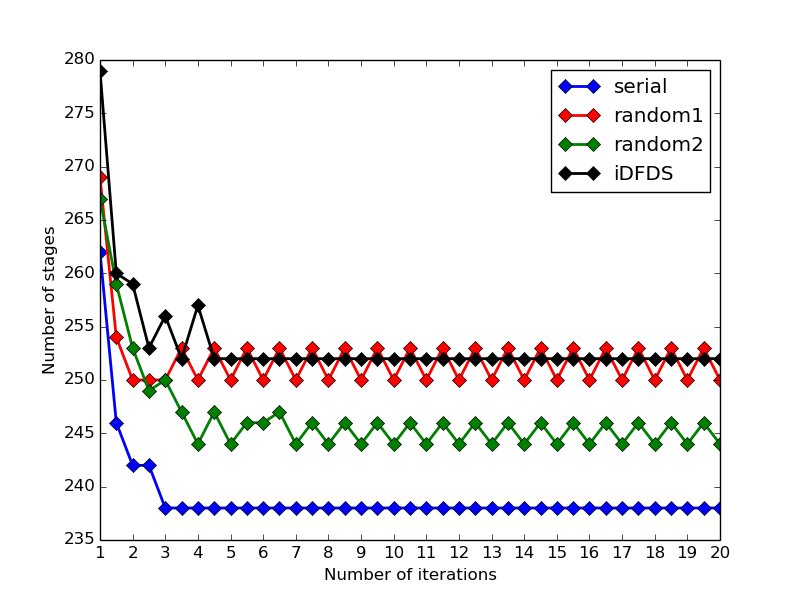
\includegraphics[width=7cm]{convergence_central_148}
    \caption{148 processors.}
  \label{convergence_central_148}
  \end{subfigure}
  \begin{subfigure}[b]{.5\textwidth}
    \centering
    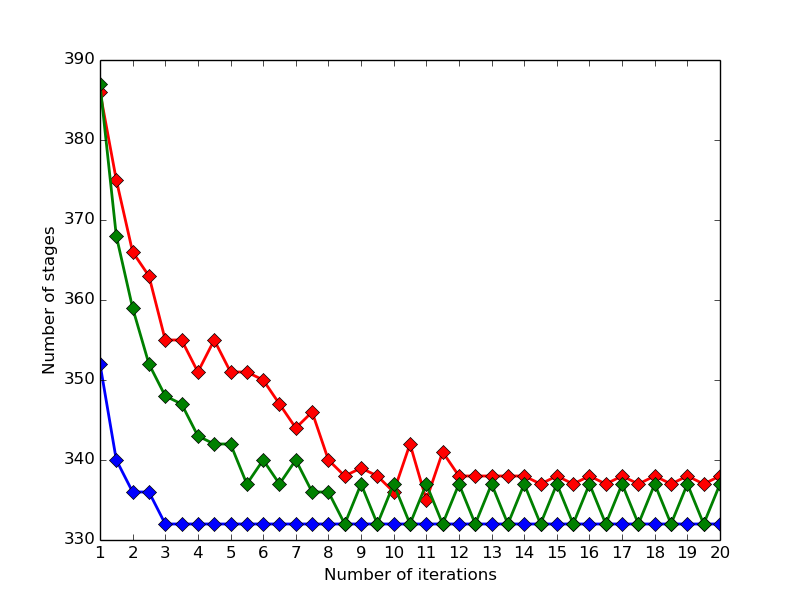
\includegraphics[width=7cm]{convergence_central_592}
    \caption{592 processors.}
  \label{convergence_central_592}
  \end{subfigure}
  \caption{Number of stages as a function of the number of CAP-PFB iterations.
  Half iterations correspond to backward iterations.}
\end{figure}


\subsection{Second AMR test}

In this test, the mesh is given in \Cref{mesh_2}. Once the gathering of tasks is
done, each processor owns tasks that require one unit of work and tasks that
require four units of work.
\begin{figure}[H]
  \centering
  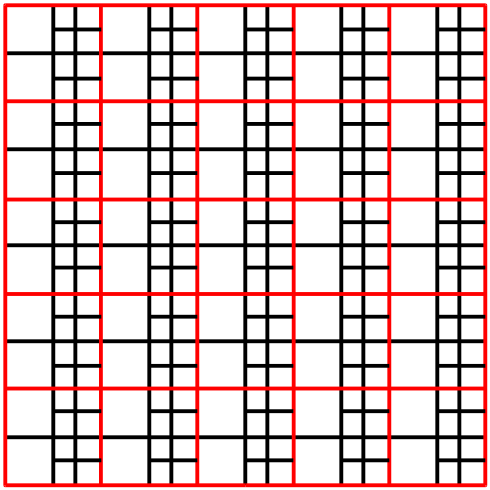
\includegraphics[width=5cm]{mesh_2}
  \caption{Mesh refined in the middle of the domain.}
  \label{mesh_2}
\end{figure}

First, we test the case where each processor owns 400 tasks (see \Cref{band_1}).
We compute the minimal number of stages in the same way as in the previous subsection. Because
the lack of symmetry of the problem, it is not obvious that this number can be reached.

\begin{table}[H]
  \begin{center}
    \caption{Number of stages required to sweep through an adapted mesh.}
    \begin{tabular}{|c|c|c|c|c|c|}
      \hline
      N.procs & Init. sweep & Init. n. stages & Best n. stages & Minimal n. stages & Iter. \\
      \hline
      $10 \times 10$ &  \emph{serial} &  40000 &  521 & 496 &  3 \\
      $10 \times 10$ & \emph{random1} &   1841 &  562 & 496 &  6 \\
      $10 \times 10$ & \emph{random2} &   1832 &  541 & 496 &  6 \\
      $10 \times 10$ &   \emph{iDFDS} &   1080 &  872 & 496 &  2 \\
      $20 \times 20$ &  \emph{serial} & 160000 &  882 & 616 &  2 \\
      $20 \times 20$ & \emph{random1} &   3488 &  882 & 616 &  3 \\
      $20 \times 20$ & \emph{random2} &   3435 &  882 & 616 &  5 \\
      $20 \times 20$ &   \emph{iDFDS} &   1851 & 1109 & 616 & 11 \\
      \hline
    \end{tabular}
    \label{band_1}
  \end{center}
\end{table}

Once again \emph{serial} gives the best results. \emph{iDFDS} performs
significantly worse than the other sweeps. In \Cref{band_2}, we show the results
when each processor owns 160 tasks.

\begin{table}[H]
  \begin{center}
    \caption{Number of stages required to sweep through an adapted mesh after
    gathering of the tasks associated to the refine cells.}
    \begin{tabular}{|c|c|c|c|c|c|}
      \hline
      N.procs & Init. sweep & Init. n. stages & Best n. stages & Minimal n. stages & Iter. \\
      \hline
      $10 \times 10$ &  \emph{serial} &  40000 &  522 & 512 & 11 \\
      $10 \times 10$ & \emph{random1} &   1833 &  539 & 512 & 16 \\
      $10 \times 10$ & \emph{random2} &   1736 &  536 & 512 & 20 \\
      $10 \times 10$ &   \emph{iDFDS} &   1225 &  553 & 512 & 19 \\
      $20 \times 20$ &  \emph{serial} & 160000 &  884 & 652 &  2 \\
      $20 \times 20$ & \emph{random1} &   3108 &  922 & 652 & 10 \\
      $20 \times 20$ & \emph{random2} &   3117 &  905 & 652 &  6 \\  
      $20 \times 20$ &   \emph{iDFDS} &   2290 &  898 & 652 & 14 \\
      \hline
    \end{tabular}
    \label{band_2}
  \end{center}
\end{table}

\emph{iDFDS} performs much better than in the previous case. \emph{serial} is
almost unaffected by the gathering but the number of stages is not optimal.
In \Cref{convergence_band}, we show the convergence of CAP-PFB. 

\begin{figure}[H]
  \begin{subfigure}[b]{.5\textwidth}
    \centering
    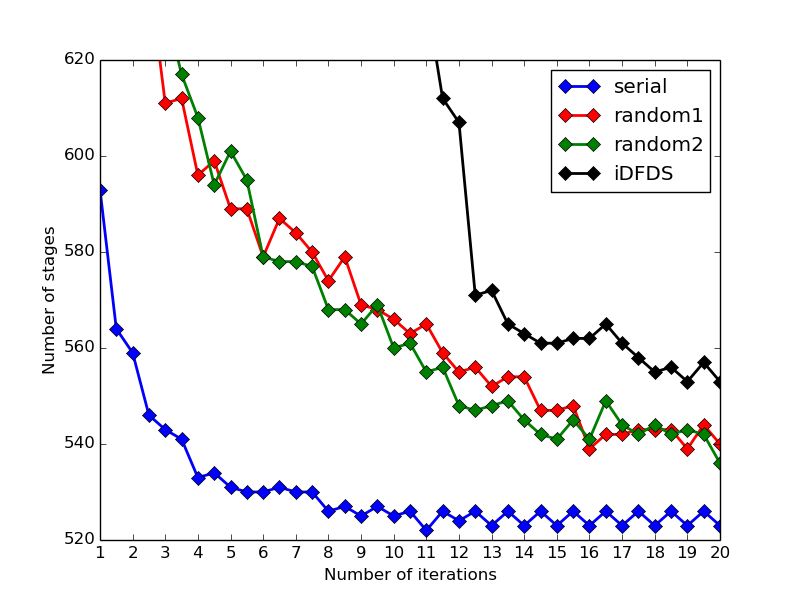
\includegraphics[width=7cm]{convergence_band_20_20}
    \caption{$10\times 10$ processors.}
    \label{cb_10_10}
  \end{subfigure}
  \begin{subfigure}[b]{.5\textwidth}
    \centering
    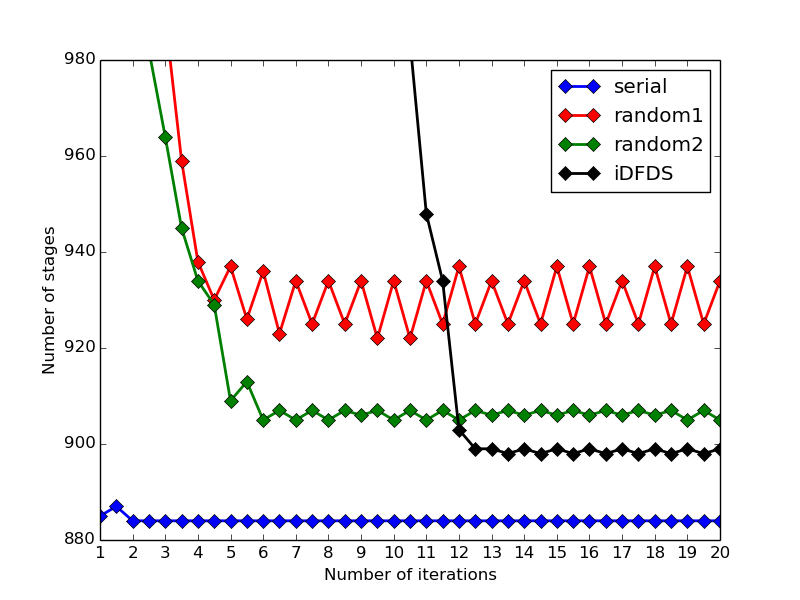
\includegraphics[width=7cm]{convergence_band_40_40}
    \caption{$20\times 20$ processors.}
  \end{subfigure}
  \caption{Number of stages as a function of the number of CAP-PFB iterations.
  Half iterations correspond backward iterations. Different colors correspond to
  different initial scheduling.}
  \label{convergence_band}
\end{figure}
 
We can see in \Cref{cb_10_10} that except for \emph{serial}, it is hard to know
if CAP-PFB has converged. It is probable that \emph{random2} and \emph{iDFDS} could be
improved and thus, the better sweep produced by \emph{serial} could be the
result of a faster convergence. Once again \emph{serial} converges faster and
more smoothly than the other methods (\emph{iDFDS} oscillations cannot be seen
on this plot).

\section{Conclusions} \label{conclusions}

In this paper, we have recalled the CAP-PFB algorithm and we have shown how it
can be applied on adaptively refined meshes. Then, we compared the sweeps
produced by CAP-PFB on uniform and adapted meshes using different initial
sweeps. On uniform meshes, CAP-PFB was shown to find an optimal sweep
independently of the initial sweep. On AMR meshes, the heuristic produced
different results given different initial sweeps but surprisingly, using an
initial sweep requiring less stages does not give the best results. The
\emph{serial} initial sweep outperformed all the other initial sweeps and it was
able to find the optimal sweep for one of the two AMR test cases when the tasks
are gathered. These results showed that the number of stages of a sweep is not
important in the choice of an initial sweep for CAP-PFB. When choosing an
initial sweep, the interaction of the sweeps along different directions is at
least as important as the sweep along each direction. Future works include using
CAP-PFB for real 2D and 3D applications and to study different initial sweeps.


%%%%%%%%%%%%%%%%%%%%%%%%%%%%%%%%%%%%%%%%%%%%%%%%%%%%%%%%%%%%%%%%%%%%%
\setlength{\baselineskip}{12pt}

\bibliographystyle{mc2015}
\bibliography{database}

%%%%%%%%%%%%%%%%%%%%%%%%%%%%%%%%%%%%%%%%%%%%%%%%%%%%%%%%%%%%%%%%%%%%%

\end{document}
